\documentclass[10pt,a4paper]{article}
\usepackage[textwidth=18cm,textheight=25cm]{geometry}
\usepackage[pdftex]{graphicx}
\usepackage{multirow}
% cv-custom.tex
%
% Custom macro commands and packages
% for formatting a Curriculum Vitae.
%
% Author: Matthew Earnshaw <matt@earnshaw.org.uk>
% Inspired by http://www.cv-templates.info/2009/03/professional-cv-latex/

\pagestyle{empty}

% Packages
\usepackage[usenames,dvipsnames]{color} % For custom colours
\usepackage{titlesec} % For custom section headings
\usepackage{mdwlist} % For compact lists
\usepackage[pdftex]{hyperref}
\usepackage{marvosym} % For icons

% Hyperlink colour and style
\definecolor{linkcolour}{rgb}{0,0.2,0.6}
\hypersetup{colorlinks,breaklinks, urlcolor=linkcolour, linkcolor=linkcolour}

% Custom colour
\definecolor{lgray}{gray}{0.4}

% Custom list bullet
\renewcommand{\labelitemi}{$\succ$}

% Header commands
\newcommand{\name}[1]{\LARGE\textbf{#1}}
\newcommand{\address}[1]{\color{lgray}{#1}}
\newcommand{\tel}[1]{\Large\Telefon~\small{#1}}
\newcommand{\email}[1]{\Large\Letter~\href{mailto:#1}{\small{#1}}}
\newcommand{\web}[2]{\Large\Mundus~\href{#1}{\small{#2}}}
	
% Section headings
\titleformat{\section}{\large\scshape\raggedright}{}{0em}{}[\titlerule]
\titlespacing{\section}{0pt}{0.6cm}{5pt}
% Note: Create an environment for sections ?

% Full width tables
\newenvironment{ftabular}[1]
{\begin{tabular*}{0.95\textwidth}{@{\extracolsep{\fill}}#1}}
{\end{tabular*}}

\usepackage[utf8]{inputenc}

\begin{document}
\footnotesize
\fontfamily{ptm}

\section{\sc P{\footnotesize ERSONAL} D{\footnotesize ETAILS}}

\begin{tabular}{ l l l }
\vspace{0.5 mm}\\
\multirow{8}{*}{\fbox{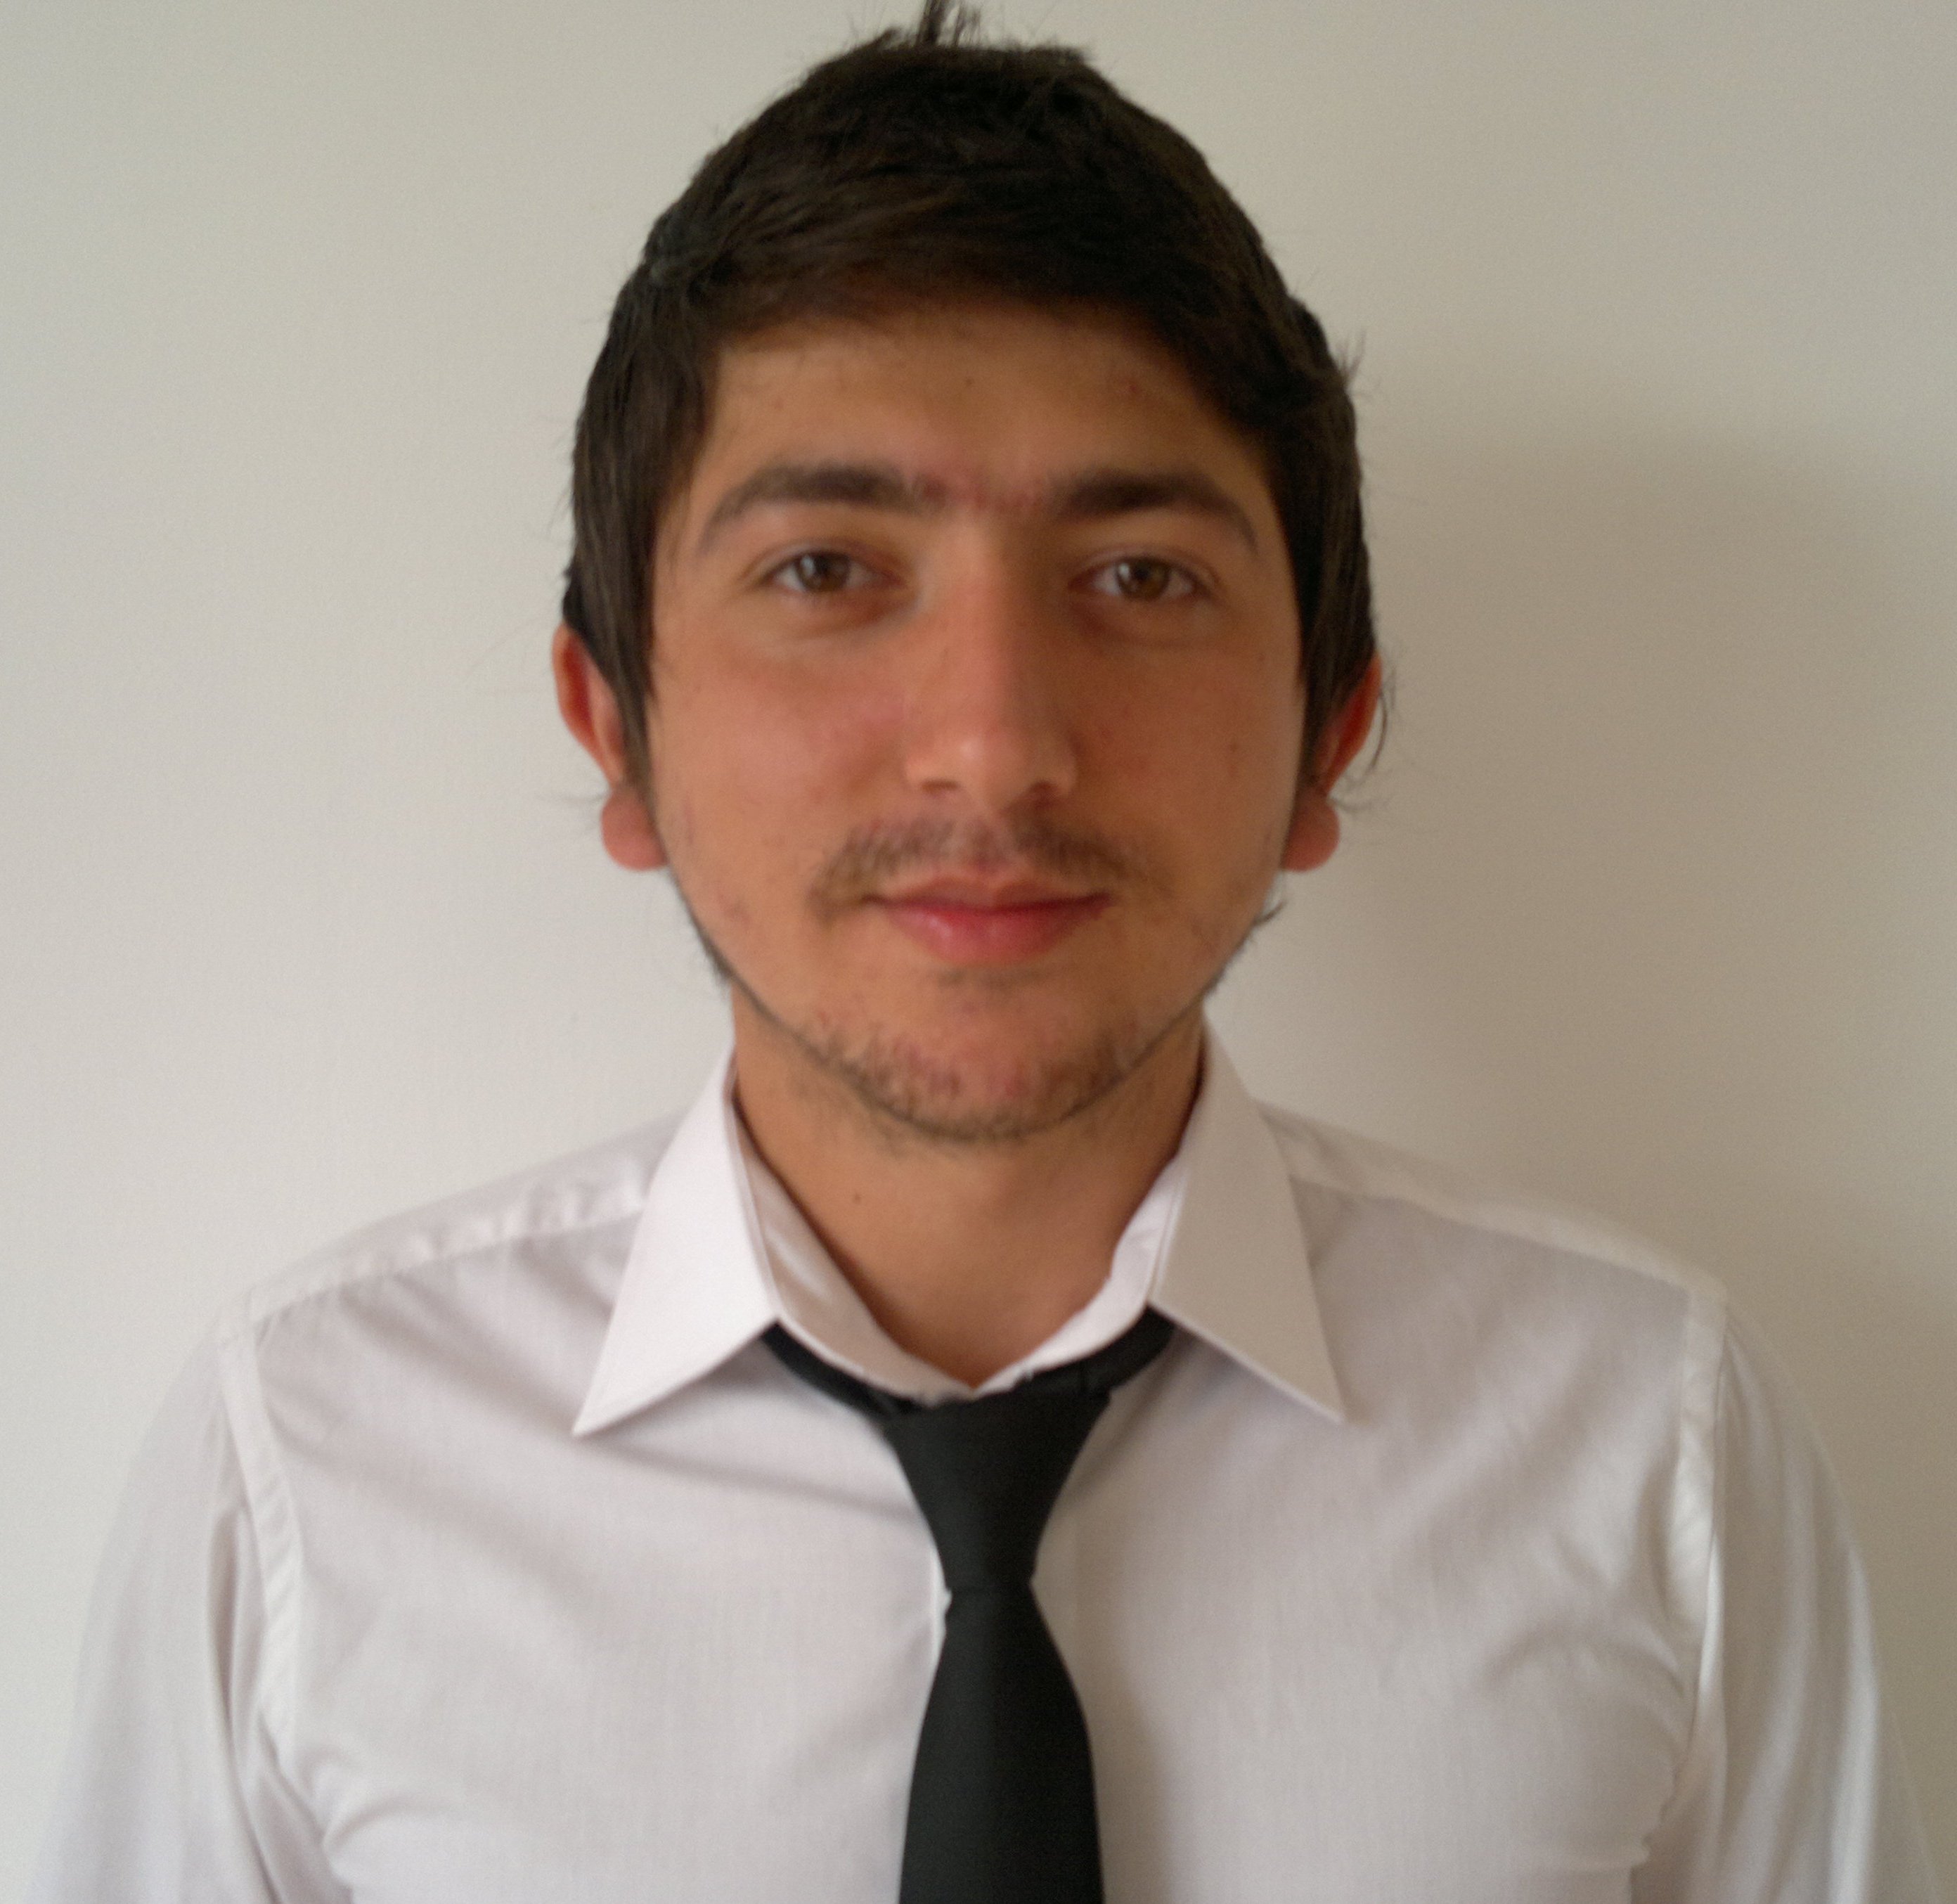
\includegraphics[height=25mm,width=25mm]{semih.jpg}}}
& {\Huge\name{Semih  Özköroğlu}}& Date: \small{08/11/2012}\\
\vspace{1 mm}\\
& \textbf{Address :} \address{Güven mah. Taşlık sok. No:21 Daire:4 Güngören/İSTANBUL} & \web{http://sozkoroglu.me}{sozkoroglu.me}\\
& \textbf{Date of Birth :} \address{18.11.1989} & \email{sem@bil.omu.edu.tr}\\
& \textbf{Marital Status :} \address{Single} & \tel{0506 3474727}\\
& \textbf{Military Service  :} \address{Suspended 01.08.2014} & \\
& \textbf{Disability :} \address{No} & \\
\end{tabular}

\section{\sc E{\footnotesize DUCATION} D{\footnotesize ETAILS}}
\hspace*{1in}\begin{tabular}{lr}
\vspace{0.5 mm}\\
\textbf{Education Level :} & University /\textbf{Graduated with Third Degree} \\
\vspace{0.5 mm}\\
\textbf{University :} & Samsun 19 Mayıs Üniversitesi \\
\textbf{Faculty/Institute :} & Engineering Faculty \\
\textbf{Section :} & Computer Engineering \\
\textbf{Learning Type / Language :} & Formal Education/Turkish \\
\textbf{Grading System / Graduation Degree :} & 100 / 77.31 \\
\textbf{Start / Graduation Date :} & September -2009 / June -2012\\
\vspace{0.5 mm}\\
\textbf{High School Type / Section :} & Normal Lyceum / Science\\
\textbf{Learning Type / Language :} & Formal Education/Turkish\\
\textbf{High School Name :} & İzzet Ünver Lisesi\\
\textbf{Grading System / Graduation Degree :} & 100 / 83.50\\
\textbf{Start / Graduation Date :} & September - 2004 / June-2007\\
\vspace{0.5 mm}\\
\end{tabular}

\underline{\textbf{Foreign Language}}
\vspace{0.5 mm}\\
\begin{itemize}
  \item{\textbf{Language :} English}
  \begin{itemize}
    \item{\textbf{General :} Middle}
    \item{\textbf{Reading :} Good}
    \item{\textbf{Writing :} Middle}
    \item{\textbf{Speaking :} Beginner}
  \end{itemize}
\end{itemize}

\section{\sc P{\footnotesize ROFESSIONAL} E{\footnotesize XPERIENCE}}
\begin{ftabular}{r|p{14cm}}
\textsc{November – 2011} & \textbf{OMU Faculty of Engineering - Samsun} \\
\vspace{0.5 mm}\\
 & \textbf{Sector – Section Position :} Computer / IT / Internet - Maintenance and Repair - Administrative Assistant\\
 & \textbf{Job Description :} I worked maintenance,update,design of Engineering Faculty Web Service that based on Wordpress.\\
 & \textbf{Reason for Leaving :} I graduated from school\\

\multicolumn{2}{c}{ } \\ % Spacer 

\textsc{October-2010 June-2011} & \textbf{OMU Industrial Engineering – Samsun} \\
\vspace{0.5 mm}\\
 & \textbf{Sector – Section Position :} Computer / IT / Internet - Science\\
 & \textbf{Job Description  :} Maintenancing computer, controlling network connections, designing web site on Department of Industrial Engineering. \\

\multicolumn{2}{c}{ } \\ % Spacer 

\textsc{November-2009 June-2010} & \textbf{Omü Distance Education Center (UZEM) - Samsun} \\
\vspace{0.5 mm}\\
 & \textbf{Sector – Section Position :} Education - Computer Science\\
 & \textbf{Job Description :} Midwifery degree completion program provides courses on the internet to midwives, midwifery degree completion program provides courses on the internet.In here i worked on video processing and support team.\\

\multicolumn{2}{c}{ } \\ % Spacer 

\textsc{July-2011} & \textbf{Dsmart - {\footnotesize İ}stanbul (Intern)} \\
\vspace{0.5 mm}\\
 & \textbf{Sector – Section Position :} Computer / IT / Internet  - Computer Engineer\\
 & \textbf{Job Description :} Redmine system installation, connection of ldap and working of privatization.\\

\multicolumn{2}{c}{ } \\ % Spacer 

\textsc{July-2010} & \textbf{Yeni Hayat Bilişim - {\footnotesize İ}stanbul (Intern)} \\
\vspace{0.5 mm}\\
 & \textbf{Sector – Section Position :} Computer / IT / Internet - Computer Engineer\\
 & \textbf{Job Description :} Searching and Using of python modules and Implement some kind of applicaitons\\

\end{ftabular}

\newpage

\section{\sc C{\footnotesize OMPETENCIES} {\footnotesize AND} S{\footnotesize KILLS}}

{\bf Programming Language (Very Good)}\\
\hspace*{0.3in}\begin{tabular}{lrrrr}
\vspace{0.5 mm}\\
  $\bullet$ C &$\bullet$ Bash &$\bullet$ Python &$\bullet$ Qt Creator &$\bullet$ Matlab\\
\end{tabular}
\vspace{0.5 mm}\\
\hspace*{0.6in}\footnotesize{``Application with Bash : \web{https://github.com/semihozkoroglu/bash-database}{Bash}``}\\
\hspace*{0.6in}\footnotesize{``Desktop Application for Smart Card System : \web{https://github.com/semihozkoroglu/kampuskart}{Python}``}\\
\hspace*{0.6in}\footnotesize{``Desktop Application for Graduation Project's Visual Interface with Qt Creator\web{https://github.com/semihozkoroglu/kampuskart}{Qt Creator}``}\\
\hspace*{0.6in}\footnotesize{``Solutions for Odtü Programming Competition : \web{https://github.com/semihozkoroglu/Workspace/tree/master/c}{C}``}\\
\hspace*{0.6in}\footnotesize{``Application of Video-Processing with Matlab : \web{https://github.com/semihozkoroglu/video-isleme}{Matlab}``}\\
\hspace*{0.6in}\footnotesize{``Image Compression Application: \web{https://github.com/semihozkoroglu/Workspace/tree/master/compress}{Matlab}``}\\

{\bf Programming Language (Good)}\\
\hspace*{0.3in}\begin{tabular}{lrrrr}
\vspace{0.5 mm}\\
  $\bullet$ C$ \# $ &$\bullet$ Ruby &$\bullet$ Rails & &\\
\end{tabular}
\vspace{0.5 mm}\\
\hspace*{0.6in}\footnotesize{``Barcode Creation and Product Tracking System \web{https://github.com/semihozkoroglu/bedix}{C$ \# $}``}\\
\hspace*{0.6in}\footnotesize{``Dictionary Data Structure: \web{https://gist.github.com/987890}{C$ \# $}``}\\
\hspace*{0.6in}\footnotesize{``Convert from Html Data to Plain Text: \web{https://gist.github.com/976957}{C$ \# $}``}\\
\hspace*{0.6in}\footnotesize{``Graduate Project's web side using with Rails Framework: \web{https://github.com/semihozkoroglu/webproje}{Ruby $ \& $ Rails}``}\\

{\bf Programming Language (Middle)}\\
\hspace*{0.3in}\begin{tabular}{lrrrr}
\vspace{0.5 mm}\\
  $\bullet$ Php &$\bullet$ Java & & &\\
\end{tabular}
\vspace{0.5 mm}\\
\hspace*{0.6in}\footnotesize{`` Facebook Application with using Heroku, ClearDB and Php: \web{https://github.com/semihozkoroglu/faceapp}{Php}``}\\
\hspace*{0.6in}\footnotesize{``Application: \web{https://apps.facebook.com/ozelkonular/}{App}``}\\
\hspace*{0.6in}\footnotesize{``Artificial Neural Networks study: \web{https://github.com/semihozkoroglu/yapaysinir}{Java}``}\\

{\bf Operating Systems}\\
\hspace*{0.3in}\begin{tabular}{lrrrr}
\vspace{0.5 mm}\\
  $\bullet$ GNU/Linux ( Good ) &$\bullet$ Windows\textregistered & & &\\
\vspace{0.5 mm}\\
\end{tabular}


{\bf Documentation Applications}\\
\hspace*{0.3in}\begin{tabular}{lrrrr}
\vspace{0.5 mm}\\
  $\bullet$ \LaTeX & & & &\\
\end{tabular}
\vspace{0.5 mm}\\
\hspace*{0.6in}\footnotesize{``Creating for Cv template script: \web{https://github.com/semihozkoroglu/cv-creator}{LaTex}``}\\
\vspace{0.5 mm}\\
\hspace*{0.6in}\footnotesize{``You can find all my works on my Github. \web{https://github.com/semihozkoroglu}{semihozkoroglu}``}\\


\section{\sc C{\footnotesize OURSES} {\footnotesize AND} S{\footnotesize EMINARS}}
\begin{ftabular}{r|p{14cm}}
\textsc{8-10 MAY 2012} & \textbf{Yeteneğe Destek Yaratıcı Ekonomiye Destek} \\
\vspace{0.5 mm}\\
 & \textbf{Company Name :}  TTNET\\

\multicolumn{2}{c}{ } \\

\textsc{25-26-27 FEBUARY 2011} & \textbf{Bilmök 7} \\
\vspace{0.5 mm}\\
 & \textbf{Company Name :}  Yeditepe Üniversitesi\\
 
\multicolumn{2}{c}{ } \\

\textsc{2-3 APRIL 2010} & \textbf{Özgür Yazılım Şenliği} \\
\vspace{0.5 mm}\\
 & \textbf{Company Name :}  Bilgi Üniversitesi\\

\multicolumn{2}{c}{ } \\

\textsc{26-28 FEBUARY 2009} & \textbf{ Bilmök 6 } \\
\vspace{0.5 mm}\\
 & \textbf{Company Name:}  Selçuk Üniversitesi\\

\end{ftabular}

\section{\sc A{\footnotesize DDITIONAL} D{\footnotesize ETAILS}}
I love Linux and i plan to improve myself in this section.

\end{document}
